\pagebreak
\section{Aufgabe 4: Support Vector Machines}
Support Vector Machines (SVMs) werden zur binären Klassifikation eingesetzt. Sie modellieren Hyperebenen, die den Datenraum in zwei zwei Teile einteilen, die jeweils eine der Zielklassen vertreten. Die Idee besteht darin, Trainingsdaten durch eine Hyperebene zu trennen, sodass ein symmetrischer Bereich um diese Hyperebene (\emph{Margin}), welcher keine Datenpunkte enthält, möglichst groß wird (\emph{Maximum Margin Hyperplane}). Da in der Praxis meist keine linear trennbaren Daten vorliegen, wird in der Trainingsphase eine Missklassifikation von Trainingsdaten toleriert. Jeder Datenpunkt, der dabei nicht außerhalb der Margin liegt oder falsch klassifiziert wird, wird entsprechend durch sogenannte Schlupfvariablen penalisiert. Dabei wird auch von einer \emph{Soft Margin} gesprochen (vgl. \cite{2015_aggarwal}).\\
\noindent \hspace*{7mm}
Ist eine lineare Trennung der Daten nicht sinnvoll, kann der \emph{Kernel Trick} angewandt werden. Dabei wird eine definierte Kernfunktion eingesetzt, die die Daten in eine höhere Dimension transformiert, indem die vorhandenen Merkmale (\emph{Input Space}) in weiteren Merkmalen vereint werden (\emph{Feature Space}). In der höheren Dimension können die Daten dann linear geteilt werden. Das Prinzip ist in den Abbildungen \ref{fig:svm_2d} und \ref{fig:svm_3d} visualisiert. Die linke Abbildung zeigt die Daten im zweidimensionalen Raum, in welchem sie nicht linear geteilt werden können. Die rechte Abbildung zeigt die transformierten, drei-dimensionalen Daten. Diese können durch eine Hyperebene geteilt werden.\\
\noindent \hspace*{7mm}
Bei SVMs werden nach der Trainingsphase nicht alle Trainingsdaten zur Klassifizierung neuer Daten genutzt. Diejenigen Datenpunkte, die zur Klassifikation betrachtet werden heißen \emph{Support Vectors}.
\begin{figure}[h]
	\centering
	\subfloat[zwei-dimensionaler Input-Space]{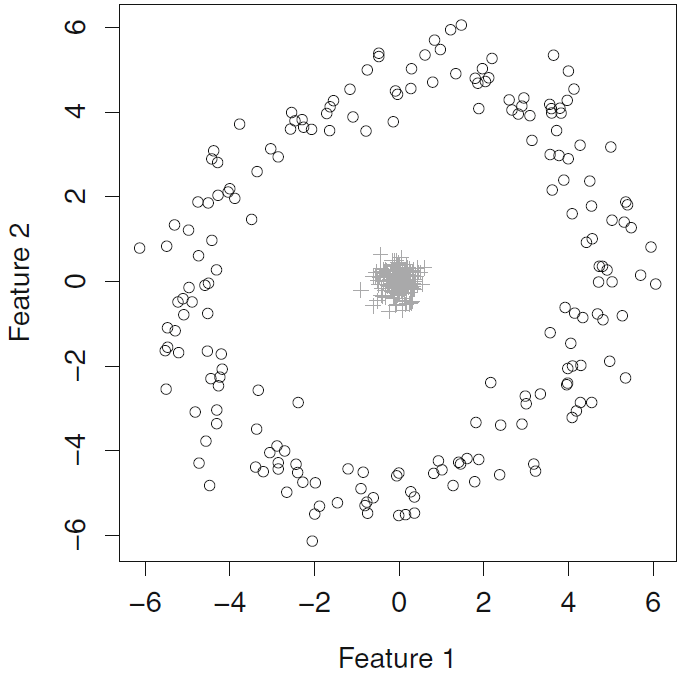
\includegraphics[width=0.40\textwidth]{Bilder/svm_2d.png}\label{fig:svm_2d}}
	\hfill
	\subfloat[drei-dimensionaler Feature-Space]{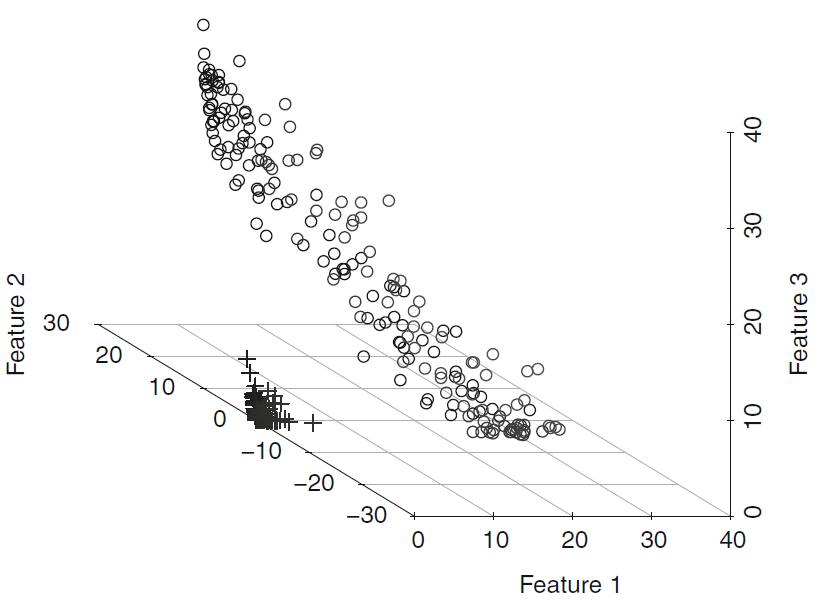
\includegraphics[width=0.40\textwidth]{Bilder/svm_3d.png}\label{fig:svm_3d}}
	\caption{Transformation der Daten durch Kernfuntionen (\cite{2018_mello_ponti})}
\end{figure}
\subsection{Beschreibung der Kernel Parameter}
Folgend sind in Tabelle \ref{tab:svm_kernel} die mathematischen Definitionen der verschiedenen Kernel gelistet. Dabei ist die Einstellung \emph{precomputed} nicht enthalten, da sie keinen definierten Kernel benutzt, sondern nur eine bereits durch einen beliebigen Kernel verarbeitete Matrix entgegennimmt. Zum Beispiel stellt $XX^{T}$ einen linearen Kernel dar. Die Kernel enthalten Parameter die im Folgenden kurz beschrieben werden.
\begin{table}[h]
	\centering
	\begin{tabular}{ll}
		\hline
		Linear (linear): &$\langle x,x^{'}\rangle$\\ \hline
		Polynomial (poly): &$(\gamma\langle x,x^{'}\rangle + r)^{d}$\\ \hline
		Radial Basis Function (rbf): &$exp(-\gamma ||x-x^{'}||^{2})$\\ \hline
		Sigmoid (sigmoid): &$tanh(\gamma \langle x,x^{'}\rangle) + r)$ \\\hline
		\hline
	\end{tabular}
	\caption{Mathematische Definitionen der Kernel}
	\label{tab:svm_kernel} 
\end{table}

\begin{description}
	\item[c (cost):]
	Dieser Parameter wird bei allen Kernen eingesetzt und gibt an, wie strikt die Margin durchgesetzt wird. Das bedeutet, dass bei kleinem $C$ eine große Margin genutzt wird, das eine höhere Anzahl an Datenpunkten innerhalb der Margin toleriert wird. Bei einem großen Wert in $C$ wird dagegen eine kleine Margin bevorzugt, da Missklassifikationen und Datenpunkte innerhalb der Margin während der Trainingsphase weniger toleriert werden (vgl. \cite{2015_aggarwal}).
	\item[gamma ($\gamma$):]
	$\gamma$ definiert den Einfluss der Trainingsdaten auf eine neue Klassifizierung. Je größer $\gamma$, desto näher müssen Trainingsdaten an dem neuen Datenpunkt liegen, um einen Einfluss zu haben. Damit steigt die Wahrscheinlichkeit des Overfittings bei einem großen $\gamma$.
	\item[degree ($d$):]
	Der Parameter $d$ gibt für den polynomialen Kernel den Grad des Polynoms an. Er kontrolliert die Flexibilität des modellierten Klassifizierers (vgl. \cite{2009_ben_hur}). Damit steigt die Wahrscheinlichkeit des Overfittings bei hohem $d$.
	\item[coef0 ($r$):]
	$r$ kann verwendet werden, um die Datenpunkte zu 'skalieren'. Das heißt, sie werden in einen anderen Wertebereich verschoben. Das kann z.B. bei dem polynomialen Kern verhindern, dass Datenpunkte, für die $\langle x,x^{'}\rangle<1$ gilt, stark von denen Datenpunkten mit $\langle x,x^{'}\rangle > 1$ separiert werden. Durch $r$ können alle Datenpunkte größer 1 gesetzt werden, sodass dieses Problem umgangen wird.
\end{description}
Die Kernel unterscheiden sich vor allem in ihrer Komplexität. Der Lineare Kernel ist der einfachste und somit robust gegen Overfitting. Er ist jedoch nicht geeignet, wenn die nicht-transformierten Daten nicht linear trennbar sind. Der polynomiale Kernel erhöht die Flexibilität bei $d>1$, sodass dessen Komplexität von Parameter $d$ bestimmt wird. Der RBF Kernel bildet einen Feature Space mit unendlich vielen Dimensionen und verhält sich ähnlich zu einem \emph{weighted-nearest-neighbour} Klassifizierer, da er mit der euklidischen Distanz ($||x-x^{'}||^{2}$) arbeitet. Daher hat auch dieser Kernel eine höhere Komplexität. Diese wird indirekt über den $\gamma$-Parameter gesteuert. Auch die Komplexität des sigmoid Kernels kann durch $gamma$ reguliert werden.
\subsection{Modellergebnis}
Bei einem Durchlauf mit $C=0.1$ und allen anderen Parametern auf Default-Einstellung zeigte der polynomiale Kernel die besten Ergebnisse. Durch das GridSearch Verfahren wurde ein X Kernel mit den Parametern a,b,c als bestes Modell geschätzt. Dieses Modell hat eine \emph{accuracy} von X
% ... blabla wieso könnten diese Parameter gewählt worden sein. Damit sollte die Frage im AB dann auch geklärt sein.!
